\cotefile{43}
\scanpage{79}
% archive sheet number: 78
% L1
\uline{\unsure{Supposons} $\dim A\geq 2$}, \unsure{on aura donc} $H^i_{\unsure{A}}(\unsure{G|\mathcal O})=0$ si $i=0,1$,

% L2--3
\deleted{Alors} $H^2(X/X-o,G)$ \unsure{est une extension de} $\operatorname{Coker}\bigl(\unsure{H^1(X,G)}\to H^1(X-o,G)\bigr)$ \unsure{par} $\operatorname{Ker}\bigl(H^2(X)\to H^2(X-o,G)\bigr)$.

% L4--7; insertion between L4 and L5 points after « propre ».
Si $G$ \unsure{est extension d'un discret par un propre}, \inserted{\unsure{et est} \uline{\unsure{simple|lisse}} \unsure{sur $k$}}, \unsure{alors par le théorème} \uline{de pureté}
\[
H^1(X,G)\to H^1(X-o,G)\quad\text{\unsure{est} \uline{surjectif}}
\]
[et si $G$ \unsure{est radiciel} ? \unsure{\ldots}]. \unsure{Quand|Quant} à $H^2(X)\to H^2(X-o,G)$

\scanpage{80}
% archive sheet number: 79
% margin note written slanted; top edge clips the first line.
\margin{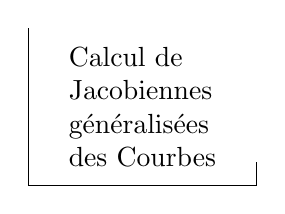
\begin{tikzpicture}\node[align=left] (t) {\unsure{Calcul de}\\Jacobiennes\\\unsure{généralisées}\\des Courbes};\draw (-1.45,1)--(-1.45,-1)--(1.45,-1)--(1.45,-.7);\end{tikzpicture}}
% D1, upper spectral-sequence scheme; the two inner terms are circled.
\diagram{\begin{tikzcd}[ampersand replacement=\&,column sep=large,row sep=small]
\text{\uuline{$\operatorname{Ext}$}}^*(\unsure{\mathscr J|J}_*,G)
  \arrow[d,phantom,"{\unsure{\prime\prime|=}\,?}"]
\& H^p\bigl(\tikz[baseline=(a.base)]{\node (a) {$\operatorname{Ext}^{\unsure{q}}(\mathscr J_*,G)$};\draw (a.center) ellipse (1.35cm and .48cm);\node at (1.1,.6) {$?$};}\bigr) \arrow[l,Leftarrow] \arrow[r,bend left=15]\&{}
\\
\phantom{H}
\& \operatorname{Ext}^p\bigl(\tikz[baseline=(b.base)]{\node (b) {$H_q(\mathscr J_*)$};\draw (b.center) ellipse (.85cm and .48cm);\node at (0,-.6) {$?$};},G\bigr) \arrow[ul,Leftarrow]\\
\deleted{H^*(X,G)}\&\&
\end{tikzcd}}
\margin{\tikz[baseline=(c.base)]{\node (c) {\unsure{ici}};\draw (c.center) ellipse (.5cm and .25cm);}}
% Top-right note is reached by an arrow from the upper circled term.
\margin{cette \unsure{suite spectrale exprime les relations entre th. de Weil et coh.} \illegible{1} \unsure{vôtre}, la \uline{\unsure{localisation}}}
% Upper right, below the spectral scheme: cancellation and interlinear addition.
\margin{\deleted{\unsure{est-ce des propriétés} \illegible{2}} \inserted{\unsure{et s'ils} \illegible{1} \unsure{fonct.} \illegible{1}} \unsure{ici} \unsure{impossible} \unsure{comparaison de 2} \illegible{1} ?? (\unsure{voir})}

% L1
$X$ de dim $1$ (\unsure{pas néc. complet, mais non singulier})

% D2 and accompanying text, L2--5
\[
H_0(\mathscr J_*)=\mathscr J^{\unsure{\bullet|'}}_{X/k}
\]
la \unsure{jacobienne de Rosenlicht} de $X$ \unsure{extension} de $Z$ par la \unsure{Albanese birationnelle} par le \unsure{quotient des groupes multiplicatifs} \inserted{\unsure{des restes}} \unsure{qui manquent à} $X$ par $\unsure{\mathbb G_m|G_m}$ \unsure{diagonal}
\[
H_{\unsure{1}}(\mathscr J_*)=
\begin{cases}
\mathbb G_m&\text{si $X$ complet}\\
0&\text{si $X$ non complet}
\end{cases}
\]

% L6 and D4
Donc si $X$ \unsure{non complet, on a}
\[
H^*(\deleted{\unsure{X,}}G)\deleted{\unsure{X}}
=\text{\uuline{$\operatorname{Ext}$}}^*(\mathscr J_*,G)
=\operatorname{Ext}^*(\mathscr J'_{X/k},G)
\]

% L7 and D5
Si $X$ est complet, \unsure{on a une suite exacte}
\diagram{\begin{tikzcd}[ampersand replacement=\&,column sep=small]
\cdots\arrow[r]\&\operatorname{Ext}^p(\mathscr J'_{X/k},G)\arrow[r]\&H^p(\unsure{G})\arrow[r]\&\operatorname{Ext}^{\unsure{p-1}}(\mathbb G_m,G)\arrow[r]\&\operatorname{Ext}^{p+1}(\mathscr J'_{X/k},G)\arrow[d]\\
\&\&\&\&\vdots
\end{tikzcd}}
\margin{\unsure{multiplication par une classe de} $\operatorname{Ext}^2(\mathscr J'_{X/k},\mathbb G_m)$}

% L8--10 and D6
\unsure{Passant à la limite inductive sur les ouverts denses de} $X$, \unsure{on trouve ainsi}, si $K=k(X)$
\[
\boxed{\operatorname{Ext}^*(\mathscr J^{\deleted{\unsure{*}}}_{K/k},G)\simeq H^*(K,G)}
\]

\scanpage{81}
% archive sheet number: 80
\deleted{\illegible{1}}
% L1--2
\unsure{Calcul de} ${\unsure{\mathscr J|J}}^{\unsure{\bullet|'}}_{A/k}$ si $A$ \unsure{est un anneau de val. discrète dont le corps résiduel} $L$ \unsure{est de degré de trans.} $1$.
\[
\coprod_{L/k}{\unsure{\mathscr S|S}}^*_L
=\underbrace{\coprod_{L/k}Z_L}_{\mathscr J^*_{L/k}}
\times\underbrace{\coprod_{L/k}\unsure{\mathbb G|G}_{m\,L}}_{\mathbb G_{m\,k}}
\times\coprod_{L/k}\mathscr S_L
\]

% L3
$U=\coprod_{L/k}\mathscr S'_L$ \unsure{est un groupe} \uline{unipotent} \uline{connexe}.

% D2: the underbraced expression continues vertically below the limits.
\[
\begin{aligned}
\operatorname{Hom}_{k\text{-gr}}(U,G)
&=\varinjlim_n\operatorname{Hom}_{L\text{-gr}}({\mathscr S'}^{(n)}_L,G_L)\\
&=\varinjlim_n\varinjlim_{\substack{C'\\\text{\unsure{ouvert}}\\\text{\unsure{non vide de} $C$}}}
\operatorname{Hom}_{C'\text{-gr}}({\mathscr S'}^{(n)}_{C'},G_{C'})\\
&=\varinjlim_{C'}\underbrace{\varinjlim_n\operatorname{Hom}_{C'\text{-gr}}({\mathscr S'}^{(n)}_{C'},G_{C'})}_{\displaystyle\operatorname{Hom}_{\substack{C'\text{-schémas}\\\text{\unsure{à sections}}\\\text{\unsure{marquées}}}}(\deleted{\unsure{G}}E^1_{C'},G_{C'})}
\end{aligned}
\]
\margin{\unsure{grâce à Rosenlicht}}
\[
\begin{aligned}
&\quad\Vert\\
&\operatorname{Hom}^{\text{\uline{\unsure{rationnels}}}}_{E^1\text{-schémas}}(C'_{E^1},G_{E^1})\\
&\quad\Vert\\
&\operatorname{Hom}^{\text{\uline{\unsure{rationnels}}}}_{E^1\text{-groupes}}
\bigl(\underbrace{\mathscr J^{\bullet}_{C'_{E^1}/\unsure{E}}}_{\mathscr J^{\bullet}_{C'/k}\times E^1},G_{E^1}\bigr)\\
&\quad\Vert\\
&\operatorname{Hom}^{\text{\uline{\unsure{rationnels}}}}_{\substack{\deleted{\unsure{k}}\\\text{\deleted{\unsure{groupes}}}\\\text{\unsure{multiplicatifs}}\\\text{\unsure{en les facteurs}}\\\text{\unsure{du groupe}}}}
(\mathscr J^{\bullet}_{C'/k}\times E^1,G)
\end{aligned}
\]
% Right-hand note is linked to the first rational-Hom line by a curved two-headed arrow.
\margin{\begin{tikzcd}[ampersand replacement=\&,column sep=small]{}\arrow[r,leftrightarrow,bend left=20]\&\text{\parbox{3.3cm}{\unsure{parmi ceux qui} \deleted{\unsure{sont}} \unsure{induisent} $0$ sur $C'_{E^1}\times_{E^1}k(\unsure{0})$ [\unsure{la fibre de l'origine de} $E^1$]}}\end{tikzcd}}
% Left auxiliary diagram, beside the vertical chain.
\diagram{\begin{tikzcd}[ampersand replacement=\&,column sep=large]
E^1_{C'}=E^1\times C'=C'_{E^1}\arrow[d] \&\\
E^1\&G_{E^1}=E^1\times G
\end{tikzcd}}
\diagram{\begin{tikzcd}[ampersand replacement=\&]
E^1\times C'\arrow[r]\&G\times C'
\end{tikzcd}}

% Bottom display.
\[
\operatorname{Hom}_{k\text{-gr}}(U,G)=
\operatorname{Hom}^{\text{\uline{\unsure{rationnels}} \unsure{en}}}_{\substack{\text{\uline{\unsure{multiplicatifs}}}\\\text{\unsure{par rapport au}}\\\text{\unsure{groupe}}}}
(\mathscr J^{\bullet}_{\unsure{L\prime|L}/k}\times E^1,G)
\]
\diagram{\begin{tikzcd}[ampersand replacement=\&]
0\arrow[r]\&U_0\arrow[r]\&U\arrow[r]\&\mathscr S'_k\arrow[r]\&0
\end{tikzcd}}
(suite splittante), donc

\scanpage{82}
% archive sheet number: 81
\[
\operatorname{Hom}_{k\text{-gr}}(U_0,G)=
\operatorname{Hom}^{\text{\uline{\unsure{rationnels}}}}_{\substack{\text{multiplicatifs}\\\text{\unsure{par rapport}}\\\text{\unsure{au facteur}}\\\text{\unsure{du groupe}}}}
({\unsure{\mathscr J|J}}^{0}_{L/k}\times E^1,G)
\]

\scanpage{84}
% archive sheet number: 83
% The heavy oblique frame, curved divider and vertical rule belong to the diagram.
\diagram{\begin{tikzcd}[ampersand replacement=\&,column sep=small,row sep=large,scale=.55,transform shape,
execute at begin picture={
\draw[line width=1.2pt] (-1.7,-3.7)--(-1.7,1.1)--(2.8,4.4);
\draw (.0,-2.5) .. controls (-.45,.0) and (-.4,.6) .. (2.9,1.6);
\draw (-1.7,-3.7)--(2.9,-.5);
\draw (2.9,-.4)--(2.9,4.4);
\draw (4.1,-1.2)--(4.1,4.2);
}]
\&\&\text{faisceaux fpqc}\&\&\\
\&\text{$k$-schémas en groupes}\arrow[ur]
\&\&\text{faisceaux fppf}\arrow[ul,"{\deleted{\unsure{u}}}"]
\&\boxed{\begin{gathered}=\text{faisceaux fpqc}\\\text{\unsure{qui commutent}}\\\text{aux }\varinjlim_{\text{\unsure{filtrés}}}\text{ d'anneaux ?}\end{gathered}}\\
\text{(\unsure{ne sont pas abéliens})}\arrow[ur,dashed,bend left]\arrow[drrr,dashed,bend right]
\&\text{$k$-gr. \unsure{pr.|qp.} qcts}\arrow[u]
\&\begin{gathered}\text{$k$-\unsure{espaces}}\\\text{loc. alg.}\end{gathered}\arrow[ul]\arrow[ur]
\&\text{gr. proalg.}\arrow[u]
\&\text{$k$-systèmes \uline{projectifs} (par injections !)}\arrow[l,dashed,dash]\\
\&\&\&\text{$k$-gr qp. qcts}\arrow[u,"{\boxed{\begin{gathered}\text{\unsure{définissable}}\\\text{\unsure{pl. fid.} ?}\end{gathered}}}"]
\&\boxed{\simeq\text{gr. proalg. \unsure{ess. affines} ?}}\\
\&\&\text{$k$-gr. alg.}\arrow[uu]\arrow[uul,"F"]\arrow[ur]\&\&
\end{tikzcd}}

% L1 below the large diagram.
$(G_i)_{i\in I}$ \unsure{définit deux faisceaux} fpqc.
\[
\begin{aligned}
\text{(i)}\quad &F(S)=\varinjlim_iG_i(S)\\
\text{(ii)}\quad &F'(S)=\bigl(\varprojlim_{\substack{\text{(en cat.}\\\text{des préschémas)}}}G_i\bigr)(S)
\end{aligned}
\]
\margin{Coïncident sur le \uline{\unsure{petit}} site fppf}
\[
\boxed{F'=u^*u_*(F)}
\]
\diagram{\begin{tikzcd}[ampersand replacement=\&]
\text{Site fpqc}\arrow[d,"u"]\\
\text{Site fppf}
\end{tikzcd}}
\[
\begin{aligned}
u^{*}_{\deleted{\unsure{*}}}&=\text{inclusion évidente des sites}\\
u_*&=\text{restriction des foncteurs}\\
u&
\end{aligned}
\]
\margin{/$u^*$ \unsure{défini par image inverse} \unsure{obj$^t$. par obj$^t$.}}

% L2--4; bracket down the left of this paragraph and list.
\noindent$\bigl[$ \unsure{Calculer les} $\operatorname{Ext}^i$ des groupes ``\unsure{élémentaires}'' sur corps alg. clos $k$, en \unsure{vérifiant que c'est pareil pour les catégories envisagées} (pour autant que ça ait un sens\ldots)
\[
\alpha_p\quad\underbrace{\mu_p\quad\unsure{\mathbb Z|Z}/p\mathbb Z}\quad\mathbb Z/\ell\mathbb Z\quad\unsure{G|\mathbb G}_a,\quad\underbrace{G_m,\quad\mathbb Z},\quad A
\]
% L5--6; second bracket at left.
\noindent$\bigl[$ Faire le calcul dans les catégories \unsure{correspondantes}, en se limitant à ce qui est annulé par un $n$ fixé.

\scanpage{85}
\mspage{132}
% archive sheet number: 84
\handwritten{[}13\handwritten{]}\quad G. Shimura -- \unsure{Redu\v{c}tion|Reduction} of algebraic varieties with respect to a discrete valuation of the basic field, Amer. J. Math. , 77 , 1955 , pp. 134-176

\handwritten{[}14\handwritten{]}\quad A. Weil -- Foundations of algebraic geometry, Amer. Math. Soc. Colloquium Publ., vol. 29, 1946 , $2^{\mathrm e}$ éd.

\handwritten{[}15\handwritten{]}\quad '' -- Variétés abéliennes et courbes algébriques, Act. Sc. et Indust. , n$^{\mathrm o}$1064, Paris, Hermann, 1948 .

\handwritten{[}16\handwritten{]}\quad '' -- Arithmetic on algebraic varieties, Ann. of Math. 78, n$^{\mathrm o}$3 , 1956 , pp. 412-444 .

\handwritten{[}17\handwritten{]}\quad '' -- Variétés kählériennes, Act. Sc. et Indust. , n$^{\mathrm o}$ 1267 , Paris, Hermann, 1958 .

\scanpage{86}
% archive sheet number: 85
% L1--2
$(Q\,\mathrm{Sch})$ \unsure{Catégorie obtenue à partir de} $(\mathrm{Sch})$ \unsure{en rendant inversibles les morphismes entiers radiciels surjectifs}

% L3--6
\unsure{Prétopologies} fppf et fpqc définies ; \unsure{on parlera de faisceaux|on parle de faisceaux} q.fpqc et q.fppf, \unsure{ce sont les} faisceaux fpqc et fppf qui \unsure{transforment morphismes entiers surj. rad. en} isom.

% Large category diagram. Thick headless strokes are kept headless.
\diagram{\begin{tikzcd}[ampersand replacement=\&,column sep=small,row sep=large,scale=.65,transform shape,
execute at begin picture={
\draw[line width=.8pt] (-6.4,4.2)--(1.4,4.2)--(1.4,3.2);
\draw (-6.4,3.7)--(-6.4,-.7)--(-4.1,-.7);
\draw (-3.8,-.7)--(-3.8,3.0)--(-1.8,3.0);
\draw (-1.8,3.0)--(-1.8,-3.5)--(1.0,-3.5)--(1.0,2.8)--(1.7,2.8);
}]
\&\&\begin{gathered}\text{faisceaux sur le}\text{ site des $k$-schémas}\\\text{qcts parfaits}\end{gathered}\arrow[dr,dash]\&\\
\begin{gathered}\text{groupes de la cat.}\text{ des $k$-schémas}\\\text{loc. qcts. parfaits}\end{gathered}\arrow[urr]\arrow[dr,dash]\arrow[dd,dash]
\&\begin{gathered}\text{\deleted{\unsure{groupes de la catégorie des}}}\\\text{\deleted{\unsure{$k$-schémas loc. qcts parfaits}}}\end{gathered}
\&\&\begin{gathered}\text{faisceaux sur le site}\\\text{\deleted{\unsure{q.fppf}} des $k$-schémas}\\\text{\deleted{loc.} qcts. parfaits}\\\text{essentiellement de}\text{ t.f. sur $k$}\end{gathered}\arrow[dd,dash]\\
\&\text{$k$-sch. en gr./rad.}\arrow[uur]\arrow[d,dash]\arrow[dr,dash]\&\&\\
\begin{gathered}\text{groupes de la catégorie}\text{ des $k$-schémas}\\\text{qcts parfaits}\end{gathered}\arrow[r,dash]
\&\begin{gathered}\text{$k$-gr. qp. qcts,}\\\text{mod rad}\end{gathered}\arrow[dr,dash]
\&\begin{gathered}\text{$k$-gr. loc. alg./radiciels}\\=\text{\deleted{\unsure{groupes algébriques}}}\\\text{\deleted{\unsure{localement}}}\end{gathered}\arrow[d,dash]\arrow[uur,dash]
\&\text{gr. proquasialg.}\arrow[d,dash]\\
\&\&\begin{gathered}\text{$k$-gr. alg./radiciels}\\\simeq\text{groupes quasi alg.}\\\text{ess de t.f.}\end{gathered}\arrow[r,dash]
\&\begin{gathered}\text{$k$-gr qp. qcts/radiciels}\\\text{\deleted{\unsure{mod rad}}}\end{gathered}
\end{tikzcd}}

\scanpage{87}
\mspage{131}
% archive sheet number: 86
\begin{center}\uline{Bibliographie}\end{center}

\handwritten{[}1\handwritten{]}\quad P. Cartier -- Questions de rationalité des diviseurs en géométrie algébrique, Bull. Soc. Math. de France , 86, 1958, pp.177-251 .

\handwritten{[}2\handwritten{]}\quad S. Lang -- Abelian varieties, Interscience tracts, New-York, \deleted{\illegible{1}} 1959 .

\handwritten{[}3\handwritten{]}\quad '' -- Diophantine geometry, Interscience tracts, New-York, 1962

\handwritten{[}4\handwritten{]}\quad '' -- Conférence au Séminaire Bourbaki, n$^{\mathrm o}$274, mai 1964 .

\handwritten{[}5\handwritten{]}\quad S. Lang and A. Néron -- Rational points on abelian varieties over function fields, Amer. J. of Math. , 81, 1, 1959 , pp. 95-118 .

\handwritten{[}6\handwritten{]}\quad A. Néron -- Arithmétique et classes de diviseurs sur les variétés algébriques, Proc. Internat. Symposium on Algebraic number theory, Tokio, 1955 , pp.139-154 .

\handwritten{[}7\handwritten{]}\quad '' -- Valeur asymptotique du nombre des points de hauteur bornée sur une courbe elliptique, Intern. Congress of Math. , Edinburgh, 1958 .

\handwritten{[}8\handwritten{]}\quad '' -- Modèles minimaux des variétés abéliennes sur les corps locaux et globaux, Publ. Inst. Hautes Et. Scientifiques, n$^{\mathrm o}$21, 1964 .

\handwritten{[}9\handwritten{]}\quad D.G. Northcott -- An inequality in the theory of arithmetic on algebraic varieties, Proc: Cambridge Philos. Soc. , 45, 1949, pp. 502-509 .

\handwritten{[}10\handwritten{]}\quad '' -- A further inequality in the theory of arithmetic on algebraic varieties; Proc. Cambridge Philos. Soc. , 45, 1949, pp. 510-518 .

\handwritten{[}11\handwritten{]}\quad P. Samuel -- Anneaux factoriels, Publ. Soc. Mat. Sao Paulo, 1963.

\handwritten{[}12\handwritten{]}\quad J-P. Serre -- Faisceaux algébriques cohérents, Annals of Math. , 61 , 2 , 1955 , pp. 197-278 .

\scanpage{89}
% archive sheet number: 88

Formulations de la \uline{dualité locale} ($F^\bullet$ constr.)

\margin{$X$ \uline{\unsure{strictmt hens}} et ``bon''\par ,\par \unsure{id|id.}}
\diagram{\begin{tikzcd}[ampersand replacement=\&,row sep=large,column sep=small,scale=.72,transform shape]
\text{(i)} \arrow[d,Rightarrow] \arrow[dd,phantom,bend right=65,"\deleted{\Downarrow}"']
 \& F^\bullet\longrightarrow D\unsure{\underline D|D}F^\bullet
 \quad\text{un \unsure{isom} \deleted{pour $F^\bullet$ constructible sur} $X$ ``bon''} \\
\text{(ii)} \arrow[d,Leftrightarrow]
 \& \begin{gathered}\text{\unsure{a)}}\ H^i_a(X,F^\bullet)\ \text{dual de}\ H^{-i}(X,\widehat F^\bullet)\\
 \deleted{\text{\unsure{b)}}\ H^i_a(X,F^\bullet)=0\ \text{\unsure{pour}}\ \forall i\ \Rightarrow\
 \unsure{H^i(X,F)=H^i(F)_{x}|H^i(X,F)\simeq H^i(F)_{x}}}\ \deleted{\unsure{\in}}\\
 \deleted{\unsure{\forall i}}
 \end{gathered} \\
\text{(iii)} \arrow[d,Leftrightarrow]
 \& H^i(X-\unsure{o|a},F^\bullet)\ \text{\unsure{dual} de}\ H^{-i-1}(X-a,\widehat F^\bullet) \\
\text{(iv)}
 \& \operatorname{Ext}^i(X;F,\lambda(G))\simeq
 \operatorname{Ext}^i(k;\mathbb R i^!(F),G)
\end{tikzcd}}
\margin{$X$ \inserted{\tikz[baseline=(l.base)]{\node (l) {local};\draw (l.center) ellipse (.55cm and .25cm);}}
hensélien ``bon'', corps résiduel $k$}

\figure{\begin{tikzpicture}\draw (0,0)--(12,.65);\end{tikzpicture}}

\vspace{5em}
\((\quad)\)

\scanpage{90}
% archive sheet number: 89

\[
H^i(U,F)=H^i(X,\mathbb R i_*(F|U))\qquad\text{dual de}
\]
\diagram{\begin{tikzcd}[ampersand replacement=\&,column sep=large,row sep=small]
U\arrow[r,"i"]\&X\\
U\arrow[r,"i'"]\&(X-a)
\end{tikzcd}}
\[
\begin{aligned}
&H^{-i}_a(X,\mathbb R i_!(\widehat F|U))\simeq
 H^{-i-1}(X-a,\mathbb R i'_!(\widehat F|U))\\
&H^{-}
\end{aligned}
\]
\[
\deleted{H^i}
\]

\margin{$a\unsure{\subset|\in} Z\subset Y\subset X$}
\diagram{\begin{tikzcd}[ampersand replacement=\&,row sep=small]
Y-Z\arrow[r,"i''"]\&X-Z\\
Y-Z\arrow[r,"k"]\&Y-a
\end{tikzcd}}
\[
\left\{\begin{aligned}
H^i_{Y-Z}(F)&=H^i(Y-Z,\mathbb R{\unsure{i'|i''}}^{!}(F|X-Z))\\
\text{\unsure{dual} de}\qquad&
H^{-i-1}(Y-a,\unsure{\mathbb R k_!}(\widehat F|(Y-Z)))
\end{aligned}\right.
\]

\diagram{\begin{tikzcd}[ampersand replacement=\&,row sep=large]
Y\arrow[r,"i"]\&X\\
Z\arrow[r,"j"]\&X
\end{tikzcd}}
\margin{$\deleted{\unsure{H^i_Y}}$}
\[
\left\{\begin{aligned}
H^i_Y(F)&=H^i(\deleted{\unsure{X|Y}}\unsure{Y|X},\mathbb R i^!(F))
\qquad\text{\unsure{dual} de}\\
H^{-i}_a(\deleted{\unsure{X|Y}}Y,\mathbb L i^*(\widehat F))
&=\deleted{\unsure{\leftarrow}}H^{-i}_a(Y,F|Y)
\end{aligned}\right.
\]
\[
\left\{\begin{aligned}
H^i_Z(F)\quad\text{\unsure{dual de}}\qquad H^{-i}_a(Z,F|Z)
\end{aligned}\right.
\]

\diagram{\begin{tikzcd}[ampersand replacement=\&,column sep=small,row sep=small,scale=.60,transform shape]
H^i_Z(F)\arrow[r]\&H^i_Y(F)\arrow[r,dash]\&H^i_{Y-Z}(F)\arrow[r]\&H^{i+1}_Z(F)\arrow[r]\&H^{i+1}_Y(F)\\
\times\&\times\&\times\&\deleted{\unsure{\times}}\ \times\&\deleted{\unsure{\times}}\ \times\\
H^{-i}_a(\widehat F|Z)\&H^{-i}_a(\widehat F|Y)\arrow[l]\&
H^{-i-1}_{\deleted{\unsure{a}}}(Y-a,\mathbb R k_!(\widehat F|Y-Z))\arrow[l]\&
H^{-i-1}_a(\widehat F|\unsure{Y|Z})\arrow[l]\&H^{-i-1}_a(\widehat F|Y)\arrow[l]
\end{tikzcd}}

\scanpage{91}
% archive sheet number: 90

\begin{flushright}
\uline{Corps de \unsure{classe} local}\par
\unsure{gèométrique|géométrique|gèomètrique|géomètrique} et dualité
\end{flushright}

\scanpage{92}
% archive sheet number: 91

$\unsure{\mathbb V|V}$ \unsure{anneau de valuation discrète, complet}, à corps résiduel $k$ parfait, \unsure{corps des fractions} $K$, \unsure{uniformisante} $\pi$.

$\mathbb V$ le schéma en anneaux sur $k$ défini par $\mathbb V$

$\mathbb K$ le ind-schéma en anneaux défini par
\[
A\rightsquigarrow\mathbb V(A)_\pi=\mathbb K(A)
\]

\margin{$\unsure{\mathscr C_S|\mathscr E_S|C_S}$}
% slanted
\margin{\unsure{Notations}}
$S=\operatorname{Spec}(\unsure{V|\mathbb V})$, on munit $S$ de la ``topologie de Weil'' définie par
\[
\left\{\begin{aligned}
&\text{\unsure{catégorie des} $S'$ plats de type fini sur $S$.}\\
&\text{descente fid. plate [\uline{\unsure{ou fid. plt. finie} ???}]}
\end{aligned}\right.
\]
% slanted
\margin{\unsure{y-a-t-il lieu de prendre} $S'$ \unsure{simple} sur $S$? Non, \unsure{bien on va perdre les|bien on peut prendre les} \unsure{groupes|gr.} \unsure{infinitésimaux}, $S'$ \unsure{tel que} $S'_0$ \unsure{soit} \deleted{\unsure{réduit}} \unsure{réduit}?? Peut-être\unsure{\ldots}}

$C(S)=$ catégorie des faisceaux de Weil abéliens sur $S$

\unsure{Donner un} $G\in C(S)$ est un foncteur $S'\rightsquigarrow G(S')$, \unsure{soumis à des conditions d'exactitude connues}.

\unsure{On convient de} \uline{prolonger} $G$ \inserted{en $\overline G$} aux préschémas plats $S'$ quelconques sur $S$, par les conditions suivantes

\begin{enumerate}[label=(\roman*)]
\item $\overline G$ \unsure{de nature locale}
\item $\overline G$ \unsure{commute aux limites inductives d'anneaux}
\end{enumerate}

Alors \unsure{on aura} $\unsure{\overline m|=}$

\begin{enumerate}[label=(\roman*),start=3]
\item $\overline G$ \unsure{compatible avec descente par morphismes} fid. plats de présentation finie.
\end{enumerate}

Exemple : tout préschéma en gr. \inserted{\unsure{comm.} $G$} sur $S$ définit un faisceau de Weil, \unsure{dénoté par la} $=$ lettre. Si $G$ est loc. de type fini sur $S$, alors le \unsure{prolongement} can. $\overline G$ est encore ``représenté'' par le $\overline m$ $G$, i.e.
\[
\overline G(S')=\operatorname{Hom}_S(S',G).
\]

\scanpage{93}
% archive sheet number: 92

Dans la catégorie $\unsure{\mathcal C|C}(S)$, \unsure{on a les foncteurs}
$H^i(S,F)$ et $\operatorname{Ext}^{i}_{\deleted{\unsure{S}}}(S;F,G)$,
$\deleted{\unsure{\operatorname{Hom}|\operatorname{Ext}}}\ \underline{\operatorname{Ext}}^i_S(F,G)$.
\unsure{Notons à ce propos}
\[
\left\{\begin{aligned}
H^i(S,F)&=\operatorname{Ext}^i(S;\unsure{\mathbb Z|Z}_S,F)\\
\mathbb E\mathrm{xt}^{*}(S;F,G)&\Longleftarrow
 H^{\unsure{p}}(S,\underline{\operatorname{Ext}}^{\unsure{1|q}}(F,G))
\end{aligned}\right.
\]

Soit $U$ l'ouvert générique de $S$, \unsure{d'où une catégorie de faisceaux} $\mathcal C(U)$.
\unsure{On a un foncteur image directe pour} $i:U\longrightarrow S$
\[
i_*:\mathcal C(U)\longrightarrow\mathcal C(S)
\]

Quels sont les foncteurs dérivés ??

\scanpage{143}
% archive sheet number: 142
\mspage{1.}

\S\,1 \uline{Notation and terminology}: Let $A$ be a Dedekind ring and let $\overline A$ be the maximal unramified extension of $A$. Let $G_A$ be the Galois group of $\overline A$ over $A$ (fundamental group of $\operatorname{Spec} A$). Let $M$ be a \uline{finite} $G_A$-module whose order, $m=\operatorname{Card} M$, is prime to all residue class characteristics of $A$, i.e. such that $\operatorname{Card} M$ is invertible in $A$. Suppose that $G_A$ operates continuously on $M$, i.e. that some open subgroup operates trivially. If $G_A$ is \uline{infinite}, we put
\[
H^r(A,M)=H^r(G_A,M)=\lim_{\underset B\longrightarrow} H^r(G_{B/A},M),
\]
the limit being taken over all \uline{finite} unramified extensions $B/A$ with respect to the inflation maps. If $G_A$ is \uline{finite}, (which for us will occur only if $A$ is the field of real or complex numbers) we put
\[
H^r(A,M)=\underline H^r(G_A,M),
\]
where the underline denotes the ``complete'' cohomology sequence, in general non-trivial in negative dimensions.

Let $\unsure{\overset{\infty}{M}|\widetilde M}=\operatorname{Hom}_{\mathbb Z}(M,\overline A^*)$ denote the Cartier dual of $M$. Here $\overline A^*$ denotes the group of invertible elements of $\overline A$. The $m$-th roots of $1$ are present so we do indeed have a perfect duality: $M\xrightarrow{\sim}\overset{\infty}{\overset{\infty}{M}}$, $\operatorname{Card} M=\operatorname{Card}\overset{\infty}{M}$, etc.

Let $\widehat H$ denote the \unsure{Pontrjagin|Pontryagin} dual of a locally compact group $H$.

\S\,2 \uline{Local Results}: Let $k$ be a locally compact field, i.e. $k=\mathbb R$, $k=\unsure{C|\mathbb C}$, or $k$ complete with respect to a discrete valuation, with finite residue class field. By local class field theory we have a canonical map $\operatorname{inv}_k:H^2(k,\overline k^*)\longrightarrow\mathbb Q/\mathbb Z$. Hence the cup product with respect to the canonical pairing \deleted{\illegible{1}} $M\times\overset{\infty}{M}\longrightarrow\overline k^*$ gives pairings
\[
H^r(k,M)\times H^{2-r}(k,\overset{\infty}{M})\longrightarrow\mathbb Q/\mathbb Z.
\]
These turn out to be perfect dualities of finite groups, i.e. we have

\uline{Theorem 2.1}: \uline{For all} $r\in\mathbb Z$, $H^r(k,M)$ \uline{is finite, and we have}
$H^{2-r}(k,M)\xrightarrow{\sim}\widehat{H^r(k,\overset{\infty}{M})}$.

If $k=\mathbb R$ or $C$ then $G_k$ is cyclic of order $2$ or $1$ and consequently $\operatorname{Card} H^r(k,M)$ is a power of $2$ and is independent of $r$.

\uline{Theorem 2.2}: \uline{If} $k$ \uline{is non-archimedean, then}
\[
\chi(k,M)\overset{\mathrm{defn.}}{=}
\frac{\operatorname{Card} H^0(k,M)\cdot\operatorname{Card} H^2(k,M)}{\operatorname{Card} H^1(k,M)}
=\frac{1}{(A:mA)}=|m|_k,
\]
\uline{where} $A$ \uline{is the valuation ring in} $k$, \uline{and where} $|m|_k$ \uline{denotes the ``normed'' abs. value of} $m$ \uline{in} $k$.

\scanpage{144}
% archive sheet number: 143
\mspage{2.}

\uline{Theorem 2.3}: \uline{If} $A$ \uline{is the valuation ring in} $k$ \uline{and if} $M$ \uline{is a} $G_A$-\uline{module such that} $mA=A$, \uline{then} $\operatorname{Card}H^0(A,M)=\operatorname{Card}H^1(A,M)$ \uline{and} $H^2(A,M)=0$. \uline{In the duality between} $H^1(k,M)$ \uline{and} $H^1(k,\unsure{\overset{\infty}{M}|\widetilde M})$ \uline{the subgroups} $H^1(A,M)$ \uline{and} $H^1(A,\overset{\infty}{M})$ \uline{are the annihilator of each other}.

\uline{Remark}: Theorem 2.1 has been generalized by S. Shatz (Harvard Thesis, June 1962) to the case where $M$ is an arbitrary Artinian \inserted{commutative} group scheme defined over $k$, and where we take cohomology with respect to arbitrary finite extensions, not only the separable ones. \deleted{\unsure{We}\ \illegible{2}} The cohomology groups are no longer finite, but can be endowed with a canonical locally compact topology. For example if $\operatorname{char}k=p>0$, then using the exact sequences

\diagram{\begin{tikzcd}[ampersand replacement=\&,column sep=small]
0\arrow[r]\&\mu_p\arrow[r]\&\unsure{\mathbb G|G}_m\arrow[r,"p"]\&\mathbb G_m\arrow[r]\&0
\end{tikzcd},\quad
\begin{tikzcd}[ampersand replacement=\&,column sep=small]
0\arrow[r]\&\alpha_p\arrow[r]\&\mathbb G_a\arrow[r,"\unsure{P|p}"]\&\mathbb G_a\arrow[r]\&0
\end{tikzcd},\quad
\begin{tikzcd}[ampersand replacement=\&,column sep=small]
0\arrow[r]\&\mathbb Z/p\mathbb Z\arrow[r]\&\mathbb G_a\arrow[r,"\wp"]\&\mathbb G_a\arrow[r]\&0
\end{tikzcd}}

we find
\diagram{\[\begin{array}{lll}
H^0(k,\mu_p)=0&H^0(k,\alpha_p)=0&H^0(k,\mathbb Z/p\mathbb Z)=\mathbb Z/p\mathbb Z\\
H^1(k,\mu_p)=k^*/k^{*p}\ \text{(compact)}&
H^1(k,\alpha_p)=k/k^p\ \text{(locally compact)}&
H^1(k,\mathbb Z/p\mathbb Z)=k/\wp k\ \text{(discrete)}\\
H^2(k,\mu_p)=\frac1p\mathbb Z/\mathbb Z&H^2(k,\alpha_p)=0&H^2(k,\mathbb Z/p\mathbb Z)=0
\end{array}\]}

and in these cases the dualities corresponding to $\mu_p=\widetilde{\mathbb Z/p\mathbb Z}$ and $\alpha_p=\widetilde\alpha_p$ are well known, being made explicit by $\langle x,y\rangle=\operatorname{Tr}\operatorname{res}(x\frac{dy}{y})$ and $=\operatorname{Tr}\operatorname{res}(x\,dy)$ respectively.

\S\,3. \uline{Global results}: Let now $k$ be a finite extension of $\mathbb Q$ (case $(N)$) or a function field in one variable over a finite field (case $(F)$). Let $S$ be a non-empty (possibly infinite) set of prime divisors of $k$, including the archimedean primes in case $(N)$; and let $A$ be the ring of elements in $k$ which are integers at all primes \uline{not} in $S$. (For example, if $S$ is the set of \uline{all} prime divisors, then $A=k$.)

\uline{Theorem 3.1}: \uline{There is a natural exact sequence of continuous maps}

\margin{$(\overset{\infty}{M})$}
\diagram{\begin{tikzcd}[ampersand replacement=\&,column sep=small,row sep=large,scale=.58,transform shape]
0\arrow[r]\&H^0(A,\overset{\infty}{M})\arrow[r,"\alpha_0"]\&
\prod_{\unsure{P|p}\in S}H^0(k_p,\overset{\infty}{M})\arrow[r,"\beta_0"]\&
\widehat{H^2(A,M)}\arrow[r,"\gamma"]\&H^1(A,\overset{\infty}{M})\arrow[d,bend left=30,"\alpha_1"]\\
\&\&\begin{gathered}\text{\uline{and isomorphisms}}\\
H^r(A,M)\xrightarrow[\sim]{\alpha_r}\prod_{P\in S}H^{\unsure{0|r}}(k_p,M)\ \text{\uline{for}}\ r\geq3.
\end{gathered}\&\&
\mathop{\unsure{\underline{\prod}|\prod}}\limits_{P\in S}H^1(k_p,\overset{\infty}{M})\arrow[d,bend left=30,"\beta_1"]\\
0\&\widehat{H^0(A,M)}\arrow[l]\&
\coprod_{P\in S}H^2(k_p,\overset{\infty}{M})\arrow[l,"\beta_2"]\&
H^2(A,\overset{\infty}{M})\arrow[l,"\alpha_2"]\&
\widehat{H^1(A,M)}\arrow[l,"\delta"]
\end{tikzcd}}

\uline{where the symbols are explained as follows}: $k_p$ denotes the completion
